\section{Design Motivation}
\label{sec:motivation}

\subsection{Focus on Significant SDCs}
\label{sec:motivation-target}
\begin{wrapfigure}{r}{0.42\textwidth}
  \centering
  \vspace{-10pt}
  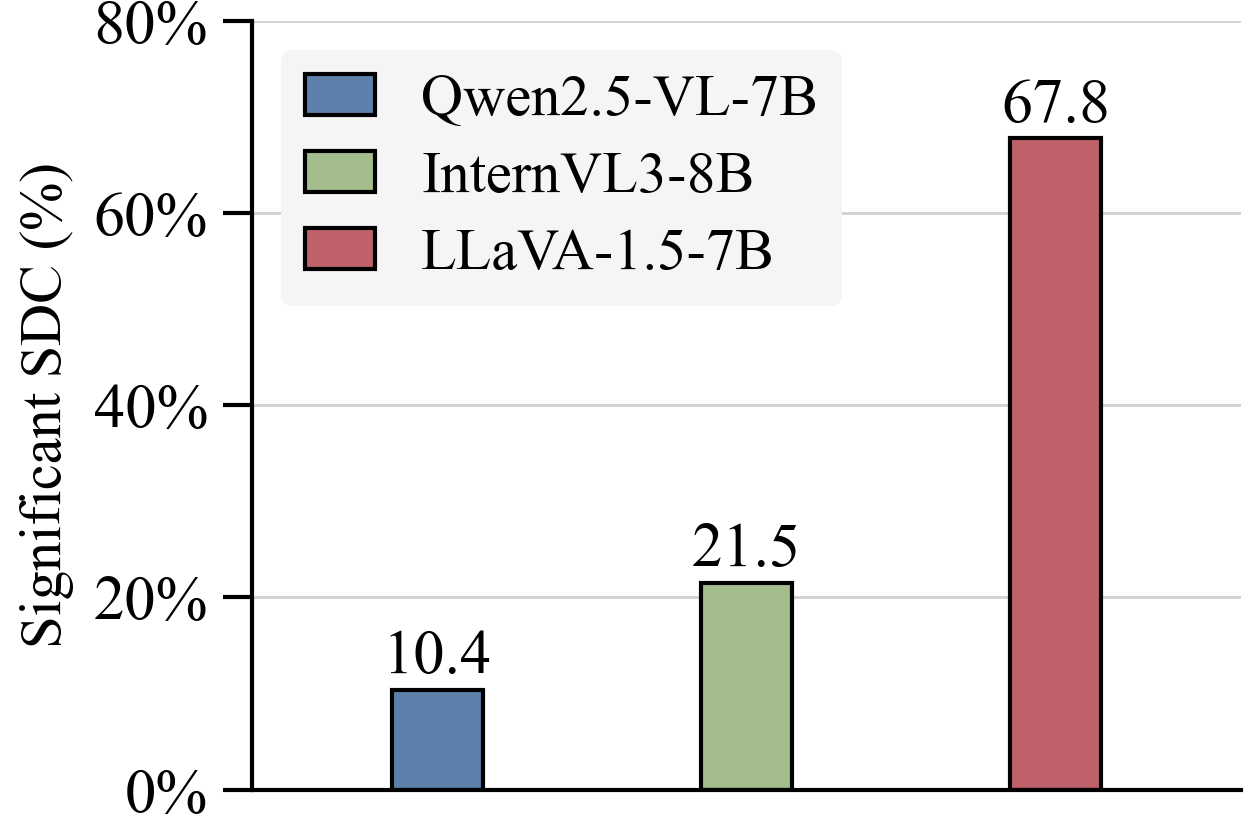
\includegraphics[width=\linewidth]{Figures/figure2_significant_SDC_share.png}
  \caption{Mean fraction of Significant SDCs among all SDCs.}
  \label{fig:2}
  \vspace{-10pt}
\end{wrapfigure}
The inherent fault tolerance of models creates a fault-masking effect that substantially raises the difficulty of SDC detection: not every hardware fault that triggers an SDC leads to catastrophic consequences. Following the definition in \S\ref{sec:intro}, an execution is marked as a \textit{Significant SDC} when its faulty output deviates from the normal output and the evaluation by an LLM-as-a-Judge (supplemented by manual review) identifies semantic deviations such as severe factual errors. As shown in Figure~\ref{fig:2}, when averaged over the three datasets, Significant SDCs account for 10.4\%, 21.5\%, and 67.8\% of all SDCs for Qwen2.5-VL-7B, InternVL3-8B, and LLaVA-1.5-7B, respectively. This indicates that most SDCs have limited semantic impact. detection should therefore focus on the small subset of Significant SDCs with severe consequences, which also reduces the number of detection targets and the subsequent error-recovery cost.

\subsection{Limitations of Numerical Deviation Detection}
\label{sec:motivation-numerical}
\begin{wrapfigure}{r}{0.42\textwidth}
  \centering
  \vspace{-10pt}
  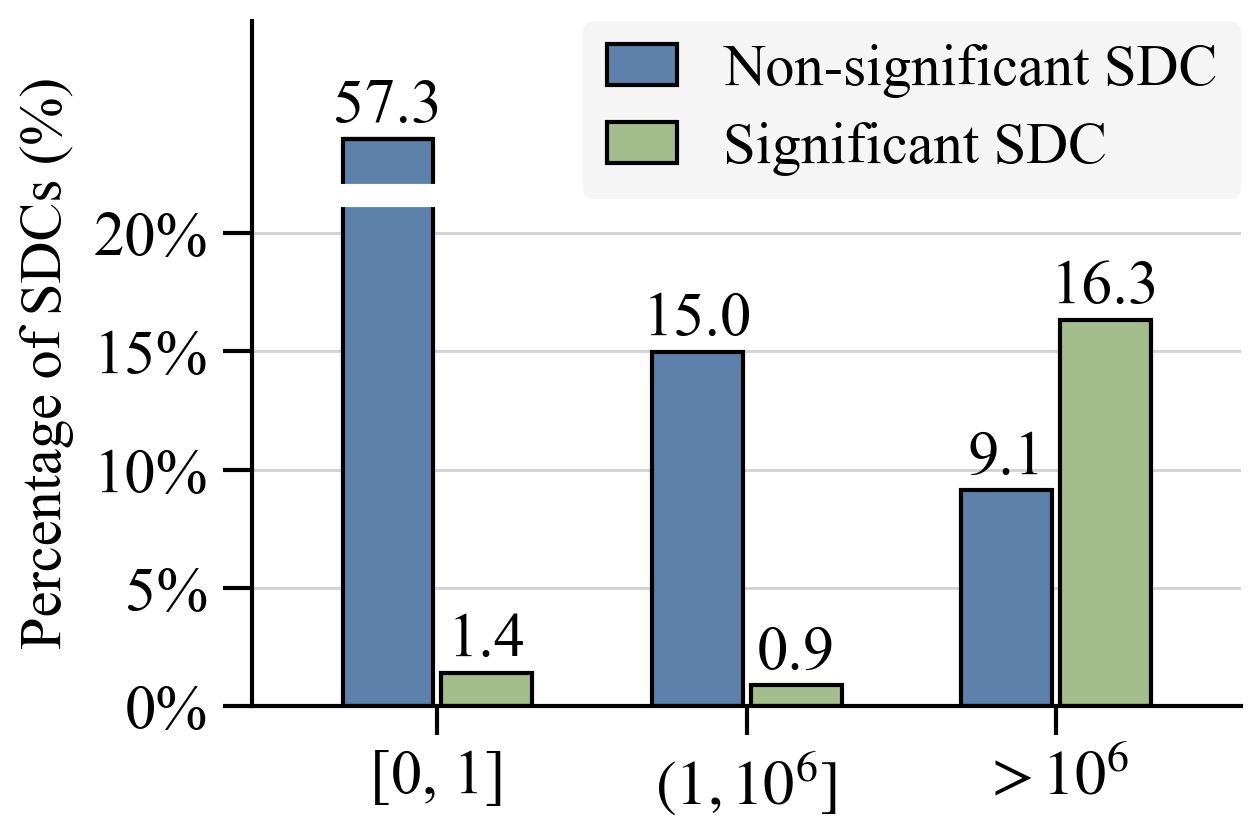
\includegraphics[width=\linewidth]{Figures/figure3_distribution_of_SDCs_by_numerical_deviation.png}
  \caption{Distribution of Non-Significant SDCs and Significant SDCs across three fault-induced value-deviation bins for finite-value faults.}
  \label{fig:3}
  \vspace{-10pt}
\end{wrapfigure}

Existing soft error detection methods typically judge fault impact by whether activations exceed normal ranges or deviate from normal distributions, implicitly assuming that a larger numerical deviation corresponds to a more severe impact. However, in LLMs, numerical deviation and output semantic damage are correlated yet not equivalent. Figure~\ref{fig:3} analyzes only faults whose injected scalar remains finite before and after the fault, and bins them by numerical deviation magnitude into three intervals: Significant SDCs already exist in the low-deviation interval, while in the high-deviation interval most faults cause no significant semantic damage. Detecting with a fixed threshold (e.g., 1) would miss 1.4\% of the Significant SDCs and raise unnecessary alarms for 24.1\% of the non-significant SDCs. Therefore, Significant SDC detection cannot rely on the magnitude of numerical deviation itself, but must characterize how faults affect the model's internal features.


